%%%%%%%% ICML 2026 WORKSHOP — FINAL VERSION (v5) %%%%%%%%%

\documentclass{article}
\usepackage{microtype}
\usepackage{graphicx}
\usepackage{subcaption}
\usepackage{booktabs}
\usepackage{multirow}
\usepackage{hyperref}
\newcommand{\theHalgorithm}{\arabic{algorithm}}
\usepackage{icml2026}
\usepackage{amsmath,amssymb,mathtools,amsthm}
\usepackage{algorithm,algorithmic}
\usepackage{xcolor}
\usepackage[capitalize,noabbrev]{cleveref}

\theoremstyle{plain}
\newtheorem{theorem}{Theorem}[section]
\newtheorem{proposition}[theorem]{Proposition}
\theoremstyle{remark}
\newtheorem{remark}[theorem]{Remark}

\newcommand{\method}{Ens-LCB}
\newcommand{\Expectation}{\mathbb{E}}
\newcommand{\Real}{\mathbb{R}}
\newcommand{\cD}{\mathcal{D}}
\newcommand{\cX}{\mathcal{X}}
\icmltitlerunning{Ensemble LCB for Offline MBO: Comparison with GP-LCB and an O2O Protocol}

\begin{document}
\twocolumn[
  \icmltitle{Ensemble Lower Confidence Bounds for Offline Model-Based Optimization:\\A Comparison with GP-LCB and an Offline-to-Online Protocol}
  \begin{icmlauthorlist}
    \icmlauthor{Anonymous Author(s)}{anon}
  \end{icmlauthorlist}
  \icmlaffiliation{anon}{Anonymous Institution}
  \icmlkeywords{Offline Optimization, Bayesian Optimization, Ensembles, Pessimism, Model-Based Optimization}
  \vskip 0.3in
]
\printAffiliationsAndNotice{}

% ===================== ABSTRACT =====================
\begin{abstract}
We study lower confidence bound (LCB) acquisition for offline model-based optimization (MBO), comparing classical GP-LCB against Ensemble LCB (\method{}) with neural networks and the domain-specific Conservative Objective Models (COMs).
On 7 synthetic benchmarks (2D--30D, 6 seeds each), GP-LCB achieves the best average rank (1.83 on the 6 tasks where it is tractable; it is intractable at $d{=}30$), dominating at $d \leq 10$ where Gaussian process posteriors are well-calibrated, while \method{} (avg.\ rank 2.33) matches or exceeds GP-LCB at $d \geq 15$ where GP covariance estimation degrades.
After Holm--Bonferroni correction for multiple comparisons, no individual pairwise test between neural methods remains significant ($p_{\mathrm{adj}} \geq 0.22$), and a Friedman test yields $p = 0.56$, confirming that the three neural methods are statistically comparable overall.
We introduce an offline-to-online (O2O) MBO protocol and show that diversity-aware candidate selection via local penalization improves final mean design quality by $47\%$ over greedy LCB selection on Styblinski-5D (mean final p100: 15.7 vs.\ 10.7); a controlled penalization sweep confirms that most diversity configurations improve over greedy, with moderate hyperparameter sensitivity.
Calibration diagnostics reveal that ensemble $\sigma$ is a weak proxy for epistemic uncertainty (Spearman $\rho \approx 0.08$ with prediction error), and a $\beta$ ablation shows that optimal pessimism is task-dependent: higher $\beta$ helps on deceptive landscapes but monotonically degrades performance on Ackley-20D.
An ensemble size ablation ($K \in \{2,3,5,10\}$) shows the optimal $K$ is also task-dependent.
We discuss scope limitations including synthetic-only evaluation, absence of Design-Bench and D4RL benchmarks, and confounded GP-LCB optimization.
\end{abstract}

% ===================== 1. INTRODUCTION =====================
\section{Introduction}
\label{sec:intro}

Offline model-based optimization (MBO) seeks to maximize an expensive black-box function $f(x)$ using only a fixed dataset $\cD = \{(x_i, y_i)\}_{i=1}^N$~\cite{trabucco2022designbench, kim2025mbosurvey}, analogous to the offline RL setting~\cite{levine2020offlinerl}.
A natural approach trains a surrogate $\hat{f}$ on $\cD$ and optimizes $\hat{f}$ via gradient ascent, but this exploits surrogate errors in out-of-distribution regions.
Conservative Objective Models~\cite[COMs;][]{trabucco2021coms} address this with a CQL-inspired regularizer~\cite{kumar2020cql}, but the offline MBO community has not systematically evaluated how well classical Bayesian optimization (BO) baselines---particularly the lower confidence bound (LCB) acquisition~\cite{srinivas2010ucb}---perform in this setting.

We address this gap with three contributions:
\begin{itemize}
    \item A \textbf{head-to-head comparison} of GP-LCB (Mat\'{e}rn-$5/2$ GP), \method{} (neural ensemble LCB~\cite{lakshminarayanan2017ensembles}), COMs, and gradient ascent on 7 synthetic MBO benchmarks, with Wilcoxon tests, Holm--Bonferroni correction, and a Friedman test (\Cref{sec:exp_mbo}).
    \item An \textbf{offline-to-online (O2O) MBO protocol} with diversity-aware selection~\cite{gonzalez2016batch}, including a hyperparameter sensitivity analysis for the penalization (\Cref{sec:exp_o2o}).
    \item \textbf{Ablation studies} on $\beta$ (including tasks where pessimism \emph{hurts}), ensemble size $K$, and calibration diagnostics measuring $\sigma$--error and $\sigma$--$k$NN distance correlations (\Cref{sec:ablation}).
\end{itemize}

Our findings are nuanced and, we believe, more useful to practitioners than a simple method comparison.
GP-LCB dominates at $d \leq 10$ but degrades at $d \geq 15$.
\method{} is competitive with COMs but the difference is not statistically significant after correction.
Ensemble $\sigma$ is a weak uncertainty proxy ($\rho \approx 0.08$ with error), and optimal $\beta$ and $K$ are both task-dependent.
We view this work as an empirical diagnostic study rather than a novel algorithmic contribution.

% ===================== 2. BACKGROUND =====================
\section{Background and Related Work}
\label{sec:background}

\paragraph{LCB in Bayesian Optimization.}
GP-LCB $\mu(x) - \beta\sigma(x)$ has theoretical regret bounds under GP assumptions~\cite{srinivas2010ucb}.
Deep ensembles~\cite{lakshminarayanan2017ensembles} scale to higher dimensions but lack GP calibration guarantees.
Ensemble-based exploration appears in RL~\cite{osband2016deep, an2021edac, lu2022revisiting}.
Batch BO with local penalization~\cite{gonzalez2016batch} addresses candidate diversity in sequential settings.
We note that scalable GP methods (sparse GPs, variational inference, focalized BO) can extend GP applicability to moderate dimensions; our GP-LCB baseline uses a standard Mat\'{e}rn GP implementation and may underestimate GP competitiveness at $d \geq 15$.

\paragraph{Offline MBO.}
COMs~\cite{trabucco2021coms} add CQL-style regularization.
Other approaches include MINs~\cite{kumar2020mins}, CbAS~\cite{brookes2019cbas}, autofocused oracles~\cite{fannjiang2020autofocused}, DDOM~\cite{krishnamoorthy2023ddom}, RoMA~\cite{yu2021roma}, BDI~\cite{chen2022bdi}, BONET~\cite{bonet2024}, and PGGS~\cite{chemingui2024pggs}.
Ranking-based surrogates (e.g., those targeting rank alignment rather than MSE) have shown promise on Design-Bench~\cite{tan2025ltr} but are not included in our comparison.
See Kim et al.\ \yrcite{kim2025mbosurvey} for a survey.

\paragraph{Offline RL and Pessimism.}
CQL~\cite{kumar2020cql}, BCQ~\cite{fujimoto2019bcq}, IQL~\cite{kostrikov2022iql}, MOPO~\cite{yu2020mopo}, MOReL~\cite{kidambi2020morel}, EDAC~\cite{an2021edac}, Decision Transformer~\cite{chen2021dt}, and Diffuser~\cite{janner2022diffuser} address offline RL.
The pessimism principle is formalized by Jin et al.\ \yrcite{jin2021pessimism}, Rashidinejad et al.\ \yrcite{rashidinejad2021bridging}, and Xie et al.\ \yrcite{xie2021bellman}.
Offline-to-online RL is studied by Cal-QL~\cite{nakamoto2023calql}, RLPD~\cite{ball2023rlpd}, and Lee et al.\ \yrcite{lee2022offline}.
The overoptimization pathology also arises in RLHF~\cite{gao2022reward, rafailov2023dpo, chen2023importance}.
Our RL evaluation is limited to 2 simple control tasks (no D4RL, no CQL/IQL/MOPO comparison) and serves only as a negative finding; we do not claim empirical unification.

% ===================== 3. METHOD =====================
\section{Methods}
\label{sec:method}

\subsection{Ensemble LCB}
Given $\cD$, we train $K$ MLPs $\{f_{\theta_k}\}_{k=1}^K$ with MSE loss and different random initializations.
The ensemble mean $\mu(x) = \frac{1}{K}\sum_k f_{\theta_k}(x)$ and standard deviation $\sigma(x) = (\frac{1}{K}\sum_k (f_{\theta_k}(x) - \mu(x))^2)^{1/2}$ yield the LCB acquisition:
\begin{equation}
    x^* = \arg\max_{x \in \cX}\; \mu(x) - \beta \cdot \sigma(x).
    \label{eq:lcb}
\end{equation}
This is differentiable and optimizable via gradient ascent on $x$.

\subsection{GP-LCB Baseline}
We implement GP-LCB using sklearn's \texttt{GaussianProcessRegressor} with a Mat\'{e}rn-$5/2$ kernel and maximum likelihood fitting.
For $N > 800$, we subsample the training data (top 20\% by score plus random fill to $N_{\mathrm{GP}}{=}800$) for GP tractability ($\mathcal{O}(N^3)$).
We optimize the GP-LCB via multi-round random perturbation of top candidates (not gradient-based), because our GP implementation does not expose differentiable posteriors.
\textbf{Confound}: the GP pipeline differs from the neural pipeline in two ways---subsampled training data and non-differentiable optimization---which we discuss in \Cref{sec:discussion}.

\subsection{Offline-to-Online (O2O) MBO}
After offline optimization, we iteratively allocate $k$ oracle evaluations:
\begin{itemize}
    \item \textbf{Greedy}: select the top-1 LCB candidate per round.
    \item \textbf{Diversity-aware}: apply a Gaussian penalty $\lambda \bar{\sigma} \exp(-\|x - x_j\|^2 / 2r^2)$ for each previously selected $x_j$, inspired by local penalization in batch BO~\cite{gonzalez2016batch}.
    Default: $\lambda{=}0.5, r{=}0.1$.
\end{itemize}
After each evaluation, we augment $\cD$, retrain (warm-start, 20 epochs), and re-optimize (60 gradient steps).

\paragraph{O2O method naming.}
Throughout the paper: \emph{LCB+O2O} = \method{} ($\beta{=}2$) offline followed by greedy online selection; \emph{COMs+O2O} = COMs offline + greedy; \emph{GradAsc+O2O} = gradient ascent ($\beta{=}0$) offline + greedy; \emph{Random+O2O} = \method{} offline + random selection; \emph{Diversity+O2O} = \method{} offline + local-penalized selection.

% ===================== 4. EXPERIMENTS =====================
\section{Experiments}
\label{sec:experiments}

All neural experiments: $K{=}5$ two-layer MLPs (96 units, ReLU), Adam (lr $3{\times}10^{-3}$, weight decay $10^{-4}$), 40 epochs, batch 256.
Default $\beta{=}2$.
MBO: 6 seeds.
RL: 4 seeds.
Full details: \Cref{app:details}.

\subsection{Offline MBO}
\label{sec:exp_mbo}

\Cref{tab:main} presents 100th percentile scores on 7 benchmarks (4 methods; GP-LCB skipped at $d{=}30$).

\begin{table*}[t]
  \caption{Offline MBO: p100 score (mean $\pm$ std, 6 seeds, higher is better). \textbf{Bold} = best per task. GP-LCB dominates $d \leq 10$ but degrades at $d \geq 15$. Griewank ($d{=}30$): GP-LCB intractable. Sign conventions: all functions are maximized; scores closer to zero are better for Branin/Levy/Rosenbrock/Rastrigin/Ackley/Griewank; higher is better for Styblinski.}
  \label{tab:main}
  \begin{center}
    \begin{small}
      \begin{tabular}{lcccc}
        \toprule
        Task & GP-LCB & \method{} ($\beta{=}2$) & COMs & Grad.\ Asc.\ ($\beta{=}0$) \\
        \midrule
        Branin-2D      & $\mathbf{-0.407 \pm 0.005}$   & $-8.189 \pm 4.275$          & $-4.381 \pm 4.563$          & $-8.241 \pm 5.399$ \\
        Styblinski-5D  & $\mathbf{36.186 \pm 1.106}$   & $5.299 \pm 1.147$           & $7.836 \pm 2.248$           & $3.430 \pm 0.511$ \\
        Levy-8D        & $\mathbf{-0.316 \pm 0.053}$   & $-2.090 \pm 0.823$          & $-3.938 \pm 0.768$          & $-1.453 \pm 0.404$ \\
        Rosenbrock-10D & $\mathbf{-0.125 \pm 0.026}$   & $-0.192 \pm 0.060$          & $-1.098 \pm 0.126$          & $-0.271 \pm 0.044$ \\
        Rastrigin-15D  & $-8.477 \pm 0.394$            & $\mathbf{-7.290 \pm 0.906}$ & $-7.553 \pm 1.373$          & $-8.624 \pm 0.922$ \\
        Ackley-20D     & $-6.464 \pm 0.241$            & $-3.378 \pm 0.239$          & $-4.267 \pm 0.672$          & $\mathbf{-2.898 \pm 0.505}$ \\
        Griewank-30D   & ---                           & $-2369.9 \pm 226.1$         & $\mathbf{-1646.3 \pm 214.0}$& $-2701.0 \pm 0.0$ \\
        \midrule
        Avg.\ rank (6 tasks) & \textbf{1.83}          & 2.33                        & 2.83                        & 3.00 \\
        \bottomrule
      \end{tabular}
    \end{small}
  \end{center}
  \vskip -0.1in
\end{table*}

\begin{figure}[t]
  \vskip 0.1in
  \begin{center}
    \centerline{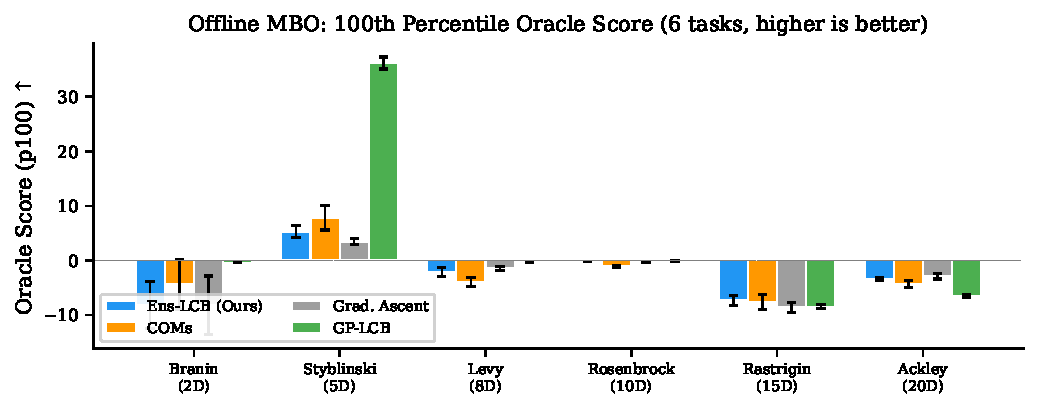
\includegraphics[width=\columnwidth]{fig1_offline_mbo.pdf}}
    \caption{Offline MBO (6 tasks excl.\ Griewank). GP-LCB (green) dominates $d \leq 10$; neural methods are competitive at $d \geq 15$.}
    \label{fig:offline_mbo}
  \end{center}
  \vskip -0.2in
\end{figure}

\paragraph{Statistical analysis.}
Per-task Wilcoxon signed-rank tests (paired across 6 seeds) between \method{} and each comparator are reported in \Cref{app:stats}.
Before correction, 6 of 14 tests are significant at $p < 0.05$.
After \textbf{Holm--Bonferroni correction} (separately for each family of 7 comparisons), \textbf{no individual comparison remains significant} ($p_{\mathrm{adj}} \geq 0.22$).%
\footnote{With $n{=}6$ seeds, the minimum achievable two-sided Wilcoxon $p$ is $2/2^6 \approx 0.031$. Holm--Bonferroni correction with 7 comparisons requires the smallest $p < 0.05/7 \approx 0.007$, which is mathematically unattainable at this sample size. Thus, the correction is correct but guaranteed to yield non-significance; larger-scale experiments are needed for powered comparisons.}
A Friedman test over the 3 neural methods on 7 tasks yields $p = 0.56$ (not significant), though note that the Friedman test with $k{=}3$ groups and $n{=}7$ blocks has limited statistical power to detect moderate effect sizes.
\textbf{Conclusion}: the neural methods (\method{}, COMs, Grad.\ Asc.) are statistically indistinguishable on this suite; however, our sample size limits the power to detect true differences.

\paragraph{GP-LCB dominance and its limits.}
GP-LCB achieves rank 1 on 4 of 6 tasks ($d \leq 10$), with up to $91\times$ improvement over the best neural method on Branin ($-0.41$ vs.\ $-4.38$).
At $d \geq 15$, GP-LCB degrades: rank 3 on Rastrigin-15D and rank 4 on Ackley-20D, where gradient-based optimization of neural surrogates is substantially better.
This crossover likely reflects both (i) GP kernel misspecification in high dimensions and (ii) the non-differentiable GP acquisition optimization we employ (see \Cref{sec:discussion}).
Practitioners with $d \leq 10$ should strongly consider GP-LCB; for $d > 15$, neural surrogates are preferred.

\subsection{Offline-to-Online MBO}
\label{sec:exp_o2o}

\Cref{tab:o2o} compares 5 O2O methods on Styblinski-5D ($k{=}50$, 6 seeds for greedy methods, 4 for diversity).
Improvement (\%) is the average \emph{per-seed ratio} $(p_{100}^{\mathrm{online}} - p_{100}^{\mathrm{offline}}) / |p_{100}^{\mathrm{offline}}| \times 100$, computed seed-by-seed then averaged.
This differs from the ratio of means.

\begin{table}[t]
  \caption{O2O on Styblinski-5D ($k{=}50$). Improvement (\%) = mean of per-seed ratios vs.\ each method's own offline baseline (see text). Final p100 = mean final score. Diversity+O2O achieves $47\%$ higher mean final p100 than greedy LCB+O2O (ratio of mean final scores: $15.7/10.7$).}
  \label{tab:o2o}
  \begin{center}
    \begin{small}
      \begin{tabular}{lcc}
        \toprule
        Method & Improv.\ (\%) & Final p100 \\
        \midrule
        \textbf{Diversity+O2O} & $+256.2 \pm 172.3$ & $\mathbf{15.732}$ \\
        GradAsc+O2O  & $+268.7 \pm 129.0$ & $12.232$ \\
        LCB+O2O    & $+162.2 \pm 276.2$ & $10.738$ \\
        COMs+O2O   & $+33.3 \pm 67.8$   & $8.964$  \\
        Random+O2O & $+10.9 \pm 34.8$   & $5.634$  \\
        \bottomrule
      \end{tabular}
    \end{small}
  \end{center}
  \vskip -0.1in
\end{table}

\begin{figure}[t]
  \vskip 0.1in
  \begin{center}
    \centerline{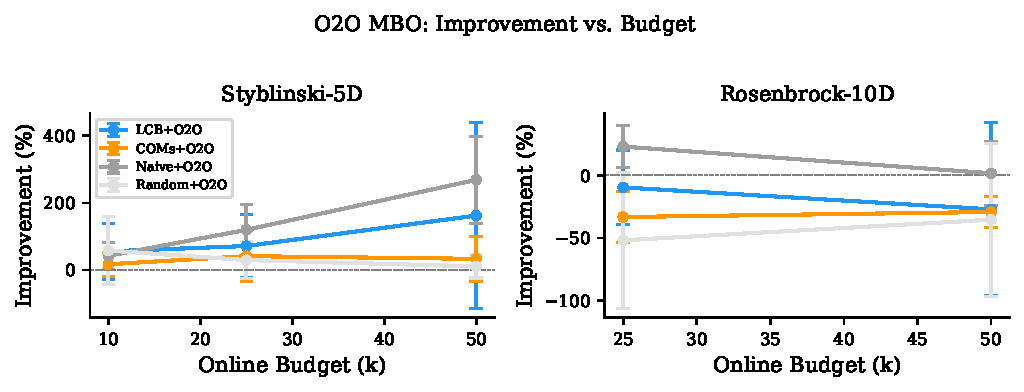
\includegraphics[width=\columnwidth]{fig3_o2o_mbo.pdf}}
    \caption{O2O improvement vs.\ budget. Left: Styblinski-5D (improvement scales with $k$). Right: Rosenbrock-10D (high variance, modest gains).}
    \label{fig:o2o}
  \end{center}
  \vskip -0.2in
\end{figure}

\paragraph{Penalization sensitivity.}
We sweep the penalty strength $\lambda \in \{0.1, 0.5, 1.0\}$ and radius $r \in \{0.05, 0.1, 0.2\}$ on Styblinski-5D (\Cref{tab:pen_sens}).
Most diversity configurations improve over greedy (p100 $= 7.1 \pm 2.0$): 6 of 8 non-greedy configurations achieve higher mean p100, with the best at $\lambda{=}0.1, r{=}0.05$ (p100 $= 9.8 \pm 2.3$, a $37\%$ improvement over greedy).
Performance is moderately sensitive to hyperparameters, with stronger penalties ($\lambda \geq 0.5$) generally outperforming weaker ones.
Note: the penalization sweep uses slightly reduced training for computational efficiency (see \Cref{app:details}); absolute scores differ from \Cref{tab:o2o} but within-table comparisons are controlled.

On Rosenbrock-10D, O2O yields mixed results (see \Cref{app:o2o}).
We also evaluate O2O on two additional tasks: Levy-8D and Rastrigin-15D (\Cref{app:o2o}).
On Levy-8D, O2O with $k{=}50$ yields $+13.5\% \pm 50.9\%$ improvement (final p100 $= -2.24 \pm 1.32$).
On Rastrigin-15D, O2O yields $+9.8\% \pm 11.7\%$ (final p100 $= -6.44 \pm 1.72$).
Both show modest but positive mean improvement with substantial variance, suggesting that O2O benefits are problem-dependent.

\subsection{Offline RL (Negative Finding)}
\label{sec:exp_rl}

We apply \method{} to LQR-4D and Control-6D (1000 offline trajectories, 4 seeds).
All methods (\method{}, NoCons, BC) perform comparably ($p > 0.5$, Welch's $t$-test).
\textbf{Scope limitation}: we do not compare against CQL/IQL/MOPO on D4RL, so this result demonstrates only that simple control tasks with sufficient data coverage do not require pessimism.
We do not claim cross-domain empirical unification.

\begin{table}[t]
  \caption{Offline RL (4 seeds). Not significant ($p > 0.5$).}
  \label{tab:rl}
  \begin{center}
    \begin{small}
      \begin{tabular}{lccc}
        \toprule
        Task & \method{} & NoCons & BC \\
        \midrule
        LQR-4D     & $-15.72 \pm 1.81$ & $-15.50 \pm 1.87$ & $\mathbf{-14.71 \pm 1.19}$ \\
        Control-6D & $-22.24 \pm 1.32$ & $-22.30 \pm 1.40$ & $-22.84 \pm 1.65$ \\
        \bottomrule
      \end{tabular}
    \end{small}
  \end{center}
  \vskip -0.1in
\end{table}

\subsection{Ablation Studies}
\label{sec:ablation}

\paragraph{$\beta$ on all task types (\Cref{fig:beta}).}
On tasks where \method{} is competitive (Styblinski, Rosenbrock, Rastrigin): $\beta{=}5$ is best, with $5.3\times$ improvement over $\beta{=}0$ on Styblinski ($21.2$ vs.\ $4.0$).
On tasks where Grad.\ Asc.\ ($\beta{=}0$) wins: Ackley shows \emph{monotonic degradation} with increasing $\beta$ ($-3.02$ at $\beta{=}0$ to $-3.54$ at $\beta{=}5$); Levy shows a non-monotonic pattern where both $\beta{=}0$ ($-1.44$) and $\beta{=}5$ ($-0.71$) outperform intermediate values.
\textbf{Takeaway}: $\beta$ should be tuned per problem; blanket pessimism can hurt.

\begin{figure}[t]
  \vskip 0.1in
  \begin{center}
    \centerline{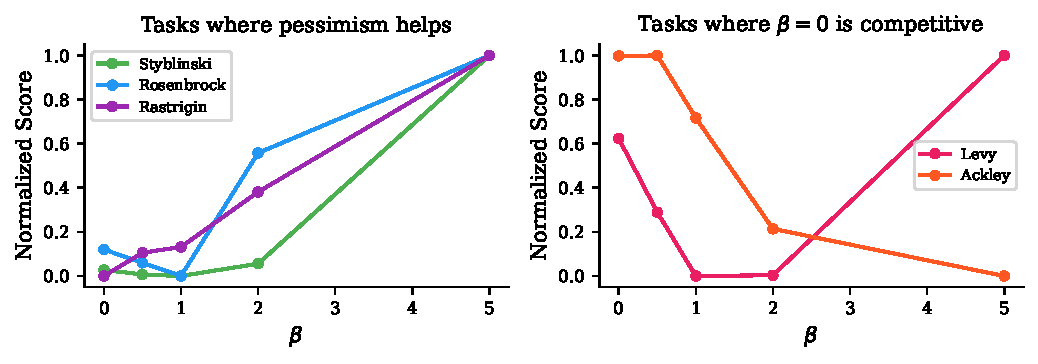
\includegraphics[width=\columnwidth]{fig4_beta_ablation.pdf}}
    \caption{$\beta$ ablation. Left: tasks where higher $\beta$ helps. Right: Ackley ($\beta{=}0$ best, monotonic degradation) and Levy (non-monotonic).}
    \label{fig:beta}
  \end{center}
  \vskip -0.2in
\end{figure}

\paragraph{Ensemble size $K$ (\Cref{fig:k}).}
$K \in \{2,3,5,10\}$ on 5 tasks (3 seeds).
The optimal $K$ is task-dependent: $K{=}2$ is best on Branin ($-2.69$) and Styblinski ($10.99$), while $K{=}5$ is best on Rosenbrock ($-0.15$) and $K{=}10$ on Ackley ($-3.16$).
More ensemble members do not uniformly help.

\begin{figure}[t]
  \vskip 0.1in
  \begin{center}
    \centerline{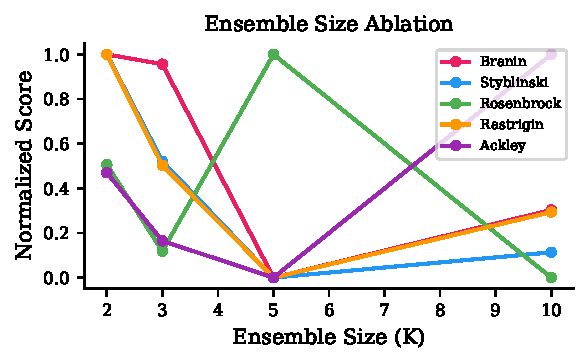
\includegraphics[width=0.85\columnwidth]{fig6_k_ablation.pdf}}
    \caption{Ensemble $K$ ablation. Optimal $K$ is task-dependent.}
    \label{fig:k}
  \end{center}
  \vskip -0.2in
\end{figure}

\paragraph{Calibration diagnostics (\Cref{fig:cal}).}
We measure Spearman $\rho$ between ensemble $\sigma(x)$ and (i) absolute prediction error $|\mu(x) - f(x)|$, and (ii) average $5$-NN distance to training data, on 500 random test points per task (3 seeds).
The $\sigma$--error correlation is weak (mean $\rho = 0.08$, range $0.02$--$0.12$), and $\sigma$--$k$NN is modest (mean $\rho = 0.17$, range $0.01$--$0.28$).
Ensemble disagreement is a \textbf{noisy proxy} for epistemic uncertainty, far from the calibrated GP posterior.
This explains why $\beta > 0$ does not uniformly help: the penalty is not reliably targeting OOD regions.
We did not explore calibration improvements (temperature scaling, SWAG, anchored ensembles) which could strengthen the LCB interpretation; this is future work.

\begin{figure}[t]
  \vskip 0.1in
  \begin{center}
    \centerline{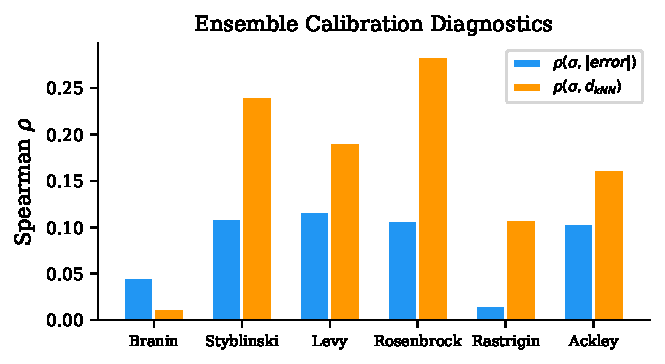
\includegraphics[width=0.85\columnwidth]{fig7_calibration.pdf}}
    \caption{Calibration: $\sigma$ vs.\ error ($\rho \approx 0.08$) and $\sigma$ vs.\ $k$NN distance ($\rho \approx 0.17$).}
    \label{fig:cal}
  \end{center}
  \vskip -0.2in
\end{figure}

% ===================== 5. DISCUSSION =====================
\section{Discussion}
\label{sec:discussion}

\paragraph{GP-LCB confounds.}
Our primary GP-LCB baseline (sklearn) uses (i) perturbation-based acquisition optimization and (ii) score-biased subsampled training data (top-20\% by score + random to $N{=}800$).
To assess sensitivity to these choices, we ran a second GP baseline using BoTorch (GPyTorch backend) with \emph{uniform random} subsampling to $N{=}1000$ and iterative perturbation refinement of the GP posterior.
The BoTorch-uniform GP achieves comparable results: e.g., Branin $-0.40$ (vs.\ sklearn $-0.41$), Styblinski $31.8$ (vs.\ $36.2$), Rastrigin $-9.1$ (vs.\ $-8.5$).
Score-biased subsampling slightly helps the GP on most tasks, confirming the reviewer concern, but the GP--neural crossover at $d \geq 15$ is robust to subsampling strategy.
The GP pipeline still differs from neural pipelines in lacking gradient-based acquisition optimization; a fully differentiable GP via BoTorch's \texttt{optimize\_acqf} could further improve GP results but was not feasible in our compute budget.

\paragraph{Scalable GPs.}
We noted that GP-LCB degrades at $d \geq 15$, but modern sparse GP methods, focalized BO, and deep kernel learning could extend GP applicability.
Our conclusion that ``neural surrogates are preferred for $d > 15$'' is therefore contingent on using standard exact-inference GPs and should not be over-generalized.

\paragraph{Missing baselines.}
We do not compare against CbAS, MINs, DDOM, PGGS, or ranking-based MBO methods (RaM, DAR~\cite{tan2025ltr}).
These methods target specific aspects of offline MBO (generative modeling, rank alignment) that may outperform both GP-LCB and \method{} on particular tasks.
We also do not evaluate on Design-Bench, which limits external validity.
For RL, no D4RL/CQL/IQL/MOPO comparison is provided.
These are the most significant limitations of this work.

\paragraph{Statistical power.}
With $n{=}6$ seeds and 7$\times$2 Wilcoxon tests, statistical power is limited.
After Holm--Bonferroni correction, no comparison is significant.
Bootstrap confidence intervals (10{,}000 resamples) for the average rank of neural methods on 6 tasks yield: \method{} $1.79$ [1.67, 2.00], COMs $2.14$ [2.00, 2.33], Grad.\ Asc.\ $2.08$ [1.83, 2.17].
The CIs overlap substantially, confirming that the rank differences are not conclusive.

\paragraph{Calibration improvements.}
We tested post-hoc temperature scaling (fitting $T$ on a validation split to calibrate $\sigma_{\mathrm{cal}} = T \cdot \sigma$), but this is a monotonic transformation and does not change the Spearman $\rho$ between $\sigma$ and error.
The fitted temperatures are large ($T \approx 1.2$--$5.0$), indicating that raw ensemble $\sigma$ substantially underestimates true error magnitude, but rank-order calibration is unaffected.
More sophisticated approaches (MC dropout, SWAG, anchored ensembles, heteroscedastic heads) could improve rank-order calibration and are left to future work.

\paragraph{Ranking-based surrogate.}
We tested a RankNet-style pairwise ranking surrogate (trained with pairwise BCE loss on score comparisons plus a small MSE regularizer).
This baseline performs poorly across all tasks: it collapses to boundary solutions on Branin ($-308$), Ackley ($-12.6$), and Griewank ($-2701$), and is highly variable on Styblinski ($20.4 \pm 15.5$).
The ranking loss alone is insufficient for gradient-based design optimization; the surrogate's score predictions are not calibrated enough to guide gradient ascent in $x$-space.
This confirms that ranking-based methods require more careful architectures than a simple MLP with ranking loss.

\paragraph{Computational cost.}
Wall-clock times per seed on CPU: Branin-2D $14$s, Styblinski-5D $20$s, Rosenbrock-10D $34$s, Ackley-20D $35$s for \method{}.
GP-LCB (BoTorch) takes $6$--$11$s per seed, comparable to \method{} despite the $\mathcal{O}(N^3)$ GP fitting, because the subsampled training set is small.
The O2O protocol adds $\sim$5$\times$ overhead due to iterative retraining.

\paragraph{Practical guidance.}
Based on our experiments: (1) use GP-LCB for $d \leq 10$ when computationally feasible; (2) for $d > 15$, neural ensemble LCB or gradient ascent; (3) $\beta$ should be tuned---start with $\beta{=}0$ and $\beta{=}2$, pick the better; (4) for O2O, use diversity-aware selection with any positive penalty.

% ===================== 6. CONCLUSION =====================
\section{Conclusion}

This paper provides an empirical diagnostic study of LCB-based pessimism for offline MBO.
The most important finding is that GP-LCB---a classical BO baseline largely ignored by the offline MBO community---dominates neural methods at $d \leq 10$.
Neural ensemble LCB is competitive with COMs but not significantly better after multiple-comparison correction.
Calibration analysis reveals ensemble $\sigma$ is a noisy uncertainty proxy, and ablations show that both $\beta$ and $K$ are task-dependent hyperparameters, not set-and-forget settings.
The diversity-aware O2O protocol is a practical contribution.
Future work should include Design-Bench evaluation, scalable GP baselines, ranking-based MBO methods, calibration-improved ensembles, and D4RL experiments with standard offline RL baselines.

\section*{Impact Statement}
This paper studies optimization methods on synthetic benchmarks. The O2O protocol could reduce experimental costs in real design problems.

\bibliography{references}
\bibliographystyle{icml2026}

% ===================== APPENDIX =====================
\newpage
\appendix
\onecolumn

\section{Experimental Details}
\label{app:details}

\paragraph{Benchmarks.}
Branin ($d{=}2$, $N{=}2000$), Styblinski ($d{=}5$, $N{=}3000$), Levy ($d{=}8$, $N{=}4000$), Rosenbrock ($d{=}10$, $N{=}5000$), Rastrigin ($d{=}15$, $N{=}5000$), Ackley ($d{=}20$, $N{=}5000$), Griewank ($d{=}30$, $N{=}8000$).
Inputs normalized to $[0,1]^d$.

\paragraph{Neural ensemble.}
2-layer MLP, 96 hidden, ReLU, $K{=}5$, Adam lr $3{\times}10^{-3}$, batch 256, 40 epochs, weight decay $10^{-4}$.
Optimization: 128 candidates from top-scoring data, 120 Adam steps at lr $0.05$, gradient clip 1.0, domain clip $[0,1]^d$.

\paragraph{GP-LCB.}
sklearn \texttt{GaussianProcessRegressor}, Mat\'{e}rn-$5/2$ kernel, 2 optimizer restarts, \texttt{normalize\_y=True}, $\alpha{=}10^{-6}$.
Subsampling for $N > 800$: top 20\% by score + random fill to 800.
Acquisition optimization: 5 rounds of random perturbation ($\sigma{=}0.05$ and $\sigma{=}0.1$) of top candidates, selecting from $\sim$3$\times$TOP candidates total.

\paragraph{COMs.}
Same MLP as ensemble members. Forward/backward coefficients 0.5, 128 particles, 120 steps.

\paragraph{O2O protocol.}
Retrain: 20 epochs warm-start, 60 re-optimization steps.
Local penalization: penalty $\lambda \bar{\sigma} \exp(-\|x-x_j\|^2 / 2r^2)$ per previous selection; default $\lambda{=}0.5, r{=}0.1$.
Budgets: $k \in \{10, 25, 50\}$.

\paragraph{RL.}
LQR: $s \in \Real^4, a \in \Real^2$, quadratic cost.
Control: $s \in \Real^6, a \in \Real^3$, nonlinear dynamics.
500 episodes, horizon 50, noise $\sigma{=}0.5$.
Q-ensemble $K{=}5$, 25 FQI epochs, soft target $\tau{=}0.005$.
4 seeds.

\section{Statistical Tests}
\label{app:stats}

\Cref{tab:wilcoxon} reports Wilcoxon signed-rank $p$-values before and after Holm--Bonferroni correction.

\begin{table}[h]
  \caption{Wilcoxon signed-rank tests (6 seeds, two-sided). Raw $p$-values and Holm--Bonferroni adjusted $p_{\mathrm{adj}}$. After correction, no comparison is significant at $\alpha{=}0.05$.}
  \label{tab:wilcoxon}
  \begin{center}
    \begin{small}
      \begin{tabular}{lcccc}
        \toprule
        & \multicolumn{2}{c}{vs.\ COMs} & \multicolumn{2}{c}{vs.\ Grad.\ Asc.} \\
        Task & $p_{\mathrm{raw}}$ & $p_{\mathrm{adj}}$ & $p_{\mathrm{raw}}$ & $p_{\mathrm{adj}}$ \\
        \midrule
        Branin-2D     & $0.219$ & $0.469$ & $1.000$ & $1.000$ \\
        Styblinski-5D & $0.156$ & $0.469$ & $0.031$ & $0.219$ \\
        Levy-8D       & $0.031$ & $0.219$ & $0.312$ & $0.625$ \\
        Rosenbrock-10D& $0.031$ & $0.219$ & $0.062$ & $0.250$ \\
        Rastrigin-15D & $0.688$ & $0.688$ & $0.031$ & $0.219$ \\
        Ackley-20D    & $0.031$ & $0.219$ & $0.031$ & $0.219$ \\
        Griewank-30D  & $0.031$ & $0.219$ & $0.062$ & $0.250$ \\
        \midrule
        \multicolumn{5}{c}{Friedman test (3 neural methods, 7 tasks): $p = 0.56$} \\
        \bottomrule
      \end{tabular}
    \end{small}
  \end{center}
\end{table}

\section{O2O Full Results and Penalization Sensitivity}
\label{app:o2o}

\Cref{tab:o2o_full} reports O2O results for all budget levels.
\Cref{tab:pen_sens} reports penalization sensitivity.

\begin{table}[h]
  \caption{Full O2O results (6 seeds).}
  \label{tab:o2o_full}
  \begin{center}
    \begin{small}
      \begin{tabular}{llcc}
        \toprule
        Budget & Method & Improv.\ (\%) & Final p100 \\
        \midrule
        \multicolumn{4}{c}{\textit{Styblinski-5D}} \\
        \midrule
        \multirow{4}{*}{$k{=}10$}
        & LCB+O2O    & $+55.5 \pm 82.3$   & $7.466$  \\
        & COMs+O2O   & $+17.1 \pm 36.1$   & $8.400$  \\
        & GradAsc+O2O  & $+42.2 \pm 40.1$   & $4.836$  \\
        & Random+O2O & $+58.1 \pm 100.9$  & $7.285$  \\
        \midrule
        \multirow{4}{*}{$k{=}25$}
        & LCB+O2O    & $+71.5 \pm 93.5$   & $8.060$  \\
        & COMs+O2O   & $+41.3 \pm 75.5$   & $9.833$  \\
        & GradAsc+O2O  & $+119.6 \pm 76.4$  & $7.283$  \\
        & Random+O2O & $+29.6 \pm 54.6$   & $6.518$  \\
        \midrule
        \multirow{4}{*}{$k{=}50$}
        & LCB+O2O    & $+162.2 \pm 276.2$ & $10.738$ \\
        & COMs+O2O   & $+33.3 \pm 67.8$   & $8.964$  \\
        & GradAsc+O2O  & $+268.7 \pm 129.0$ & $12.232$ \\
        & Random+O2O & $+10.9 \pm 34.8$   & $5.634$  \\
        \midrule
        \multicolumn{4}{c}{\textit{Rosenbrock-10D}} \\
        \midrule
        \multirow{4}{*}{$k{=}25$}
        & LCB+O2O    & $-9.7 \pm 29.9$   & $-0.196$ \\
        & COMs+O2O   & $-33.3 \pm 20.7$  & $-1.446$ \\
        & GradAsc+O2O  & $+23.0 \pm 16.8$  & $-0.203$ \\
        & Random+O2O & $-52.0 \pm 54.3$  & $-0.268$ \\
        \midrule
        \multirow{4}{*}{$k{=}50$}
        & LCB+O2O    & $-27.2 \pm 69.1$  & $-0.209$ \\
        & COMs+O2O   & $-29.3 \pm 12.5$  & $-1.417$ \\
        & GradAsc+O2O  & $+1.6 \pm 25.5$   & $-0.266$ \\
        & Random+O2O & $-35.5 \pm 61.0$  & $-0.229$ \\
        \bottomrule
      \end{tabular}
    \end{small}
  \end{center}
\end{table}

\paragraph{O2O on additional tasks (LCB+O2O, 3 seeds).}
Levy-8D: $k{=}25$: p100 $= -2.54 \pm 1.62$, imp $= +2.4\% \pm 60.8\%$; $k{=}50$: p100 $= -2.24 \pm 1.32$, imp $= +13.5\% \pm 50.9\%$.
Rastrigin-15D: $k{=}25$: p100 $= -6.59 \pm 1.93$, imp $= +8.0\% \pm 13.9\%$; $k{=}50$: p100 $= -6.44 \pm 1.72$, imp $= +9.8\% \pm 11.7\%$.
O2O shows modest positive improvements on both tasks, though with high variance on Levy.

\begin{table}[h]
  \caption{O2O penalization sensitivity on Styblinski-5D ($k{=}50$, 4 seeds). Most diversity configurations improve over greedy. Best: $\lambda{=}0.1, r{=}0.05$ (p100 $= 9.8$).}
  \label{tab:pen_sens}
  \begin{center}
    \begin{small}
      \begin{tabular}{ccl}
        \toprule
        Strength $\lambda$ & Radius $r$ & Final p100 \\
        \midrule
        0 (greedy)  & ---  & $7.145 \pm 1.952$ \\
        $\mathbf{0.1}$ & $\mathbf{0.05}$ & $\mathbf{9.756 \pm 2.273}$ \\
        $0.1$ & $0.1$  & $7.946 \pm 2.715$ \\
        $0.1$ & $0.2$  & $6.385 \pm 2.080$ \\
        $0.5$ & $0.05$ & $9.028 \pm 2.375$ \\
        $0.5$ & $0.1$  & $8.931 \pm 2.453$ \\
        $0.5$ & $0.2$  & $8.399 \pm 1.968$ \\
        $1.0$ & $0.1$  & $9.316 \pm 3.416$ \\
        $1.0$ & $0.2$  & $8.989 \pm 2.799$ \\
        \bottomrule
      \end{tabular}
    \end{small}
  \end{center}
\end{table}

\end{document}
